\documentclass[11pt,addpoints,answers]{exam}
\usepackage[margin=1in]{geometry}
\usepackage{amsmath, amsfonts}
\usepackage{enumerate}
\usepackage{graphicx}
\usepackage{titling}
\usepackage{url}
\usepackage{xfrac}
\usepackage{geometry}
\usepackage{graphicx}
\usepackage{natbib}
\usepackage{amsmath}
\usepackage{amssymb}
\usepackage{amsthm}
\usepackage{paralist}
\usepackage{epstopdf}
\usepackage{tabularx}
\usepackage{longtable}
\usepackage{multirow}
\usepackage{multicol}
\usepackage[colorlinks=true,urlcolor=blue]{hyperref}
\usepackage{fancyvrb}
\usepackage{algorithm}
\usepackage{algorithmic}
\usepackage{float}
\usepackage{paralist}
\usepackage[svgname]{xcolor}
\usepackage{enumerate}
\usepackage{array}
\usepackage{times}
\usepackage{url}
\usepackage{comment}
\usepackage{environ}
\usepackage{times}
\usepackage{textcomp}
\usepackage{caption}
\usepackage[colorlinks=true,urlcolor=blue]{hyperref}
\usepackage{listings}
\usepackage{parskip} % For NIPS style paragraphs.
\usepackage[compact]{titlesec} % Less whitespace around titles
\usepackage[inline]{enumitem} % For inline enumerate* and itemize*
\usepackage{datetime}
\usepackage{comment}
% \usepackage{minted}
\usepackage{lastpage}
\usepackage{color}
\usepackage{xcolor}
\usepackage{listings}
\usepackage{tikz}
\usetikzlibrary{shapes,decorations,bayesnet}
%\usepackage{framed}
\usepackage{graphicx}
\usepackage{booktabs}
\usepackage{cprotect}
\usepackage{xcolor}
\usepackage{verbatimbox}
\usepackage[many]{tcolorbox}
\usepackage{cancel}
\usepackage{wasysym}
\usepackage{mdframed}
\usepackage{subcaption}
\usetikzlibrary{shapes.geometric}

%%%%%%%%%%%%%%%%%%%%%%%%%%%%%%%%%%%%%%%%%%%
% Formatting for \CorrectChoice of "exam" %
%%%%%%%%%%%%%%%%%%%%%%%%%%%%%%%%%%%%%%%%%%%

\CorrectChoiceEmphasis{}
\checkedchar{\blackcircle}

%%%%%%%%%%%%%%%%%%%%%%%%%%%%%%%%%%%%%%%%%%%
% Better numbering                        %
%%%%%%%%%%%%%%%%%%%%%%%%%%%%%%%%%%%%%%%%%%%

\numberwithin{equation}{section} % Number equations within sections (i.e. 1.1, 1.2, 2.1, 2.2 instead of 1, 2, 3, 4)
\numberwithin{figure}{section} % Number figures within sections (i.e. 1.1, 1.2, 2.1, 2.2 instead of 1, 2, 3, 4)
\numberwithin{table}{section} % Number tables within sections (i.e. 1.1, 1.2, 2.1, 2.2 instead of 1, 2, 3, 4)


%%%%%%%%%%%%%%%%%%%%%%%%%%%%%%%%%%%%%%%%%%%
% Common Math Commands                    %
%%%%%%%%%%%%%%%%%%%%%%%%%%%%%%%%%%%%%%%%%%%

%%%%%%%%%%%%%%%%%%%%%%%%%%%%%%%%%%%%%%%%%%
% Custom commands                        %
%%%%%%%%%%%%%%%%%%%%%%%%%%%%%%%%%%%%%%%%%%

\newcommand{\vc}[1]{\boldsymbol{#1}}
\newcommand{\adj}[1]{\frac{d J}{d #1}}
\newcommand{\chain}[2]{\adj{#2} = \adj{#1}\frac{d #1}{d #2}}

% mathcal
\newcommand{\Ac}{\mathcal{A}}
\newcommand{\Bc}{\mathcal{B}}
\newcommand{\Cc}{\mathcal{C}}
\newcommand{\Dc}{\mathcal{D}}
\newcommand{\Ec}{\mathcal{E}}
\newcommand{\Fc}{\mathcal{F}}
\newcommand{\Gc}{\mathcal{G}}
\newcommand{\Hc}{\mathcal{H}}
\newcommand{\Ic}{\mathcal{I}}
\newcommand{\Jc}{\mathcal{J}}
\newcommand{\Kc}{\mathcal{K}}
\newcommand{\Lc}{\mathcal{L}}
\newcommand{\Mc}{\mathcal{M}}
\newcommand{\Nc}{\mathcal{N}}
\newcommand{\Oc}{\mathcal{O}}
\newcommand{\Pc}{\mathcal{P}}
\newcommand{\Qc}{\mathcal{Q}}
\newcommand{\Rc}{\mathcal{R}}
\newcommand{\Sc}{\mathcal{S}}
\newcommand{\Tc}{\mathcal{T}}
\newcommand{\Uc}{\mathcal{U}}
\newcommand{\Vc}{\mathcal{V}}
\newcommand{\Wc}{\mathcal{W}}
\newcommand{\Xc}{\mathcal{X}}
\newcommand{\Yc}{\mathcal{Y}}
\newcommand{\Zc}{\mathcal{Z}}

% mathbb
\newcommand{\Ab}{\mathbb{A}}
\newcommand{\Bb}{\mathbb{B}}
\newcommand{\Cb}{\mathbb{C}}
\newcommand{\Db}{\mathbb{D}}
\newcommand{\Eb}{\mathbb{E}}
\newcommand{\Fb}{\mathbb{F}}
\newcommand{\Gb}{\mathbb{G}}
\newcommand{\Hb}{\mathbb{H}}
\newcommand{\Ib}{\mathbb{I}}
\newcommand{\Jb}{\mathbb{J}}
\newcommand{\Kb}{\mathbb{K}}
\newcommand{\Lb}{\mathbb{L}}
\newcommand{\Mb}{\mathbb{M}}
\newcommand{\Nb}{\mathbb{N}}
\newcommand{\Ob}{\mathbb{O}}
\newcommand{\Pb}{\mathbb{P}}
\newcommand{\Qb}{\mathbb{Q}}
\newcommand{\Rb}{\mathbb{R}}
\newcommand{\Sb}{\mathbb{S}}
\newcommand{\Tb}{\mathbb{T}}
\newcommand{\Ub}{\mathbb{U}}
\newcommand{\Vb}{\mathbb{V}}
\newcommand{\Wb}{\mathbb{W}}
\newcommand{\Xb}{\mathbb{X}}
\newcommand{\Yb}{\mathbb{Y}}
\newcommand{\Zb}{\mathbb{Z}}

% mathbf lowercase
\newcommand{\av}{\mathbf{a}}
\newcommand{\bv}{\mathbf{b}}
\newcommand{\cv}{\mathbf{c}}
\newcommand{\dv}{\mathbf{d}}
\newcommand{\ev}{\mathbf{e}}
\newcommand{\fv}{\mathbf{f}}
\newcommand{\gv}{\mathbf{g}}
\newcommand{\hv}{\mathbf{h}}
\newcommand{\iv}{\mathbf{i}}
\newcommand{\jv}{\mathbf{j}}
\newcommand{\kv}{\mathbf{k}}
\newcommand{\lv}{\mathbf{l}}
\newcommand{\mv}{\mathbf{m}}
\newcommand{\nv}{\mathbf{n}}
\newcommand{\ov}{\mathbf{o}}
\newcommand{\pv}{\mathbf{p}}
\newcommand{\qv}{\mathbf{q}}
\newcommand{\rv}{\mathbf{r}}
\newcommand{\sv}{\mathbf{s}}
\newcommand{\tv}{\mathbf{t}}
\newcommand{\uv}{\mathbf{u}}
\newcommand{\vv}{\mathbf{v}}
\newcommand{\wv}{\mathbf{w}}
\newcommand{\xv}{\mathbf{x}}
\newcommand{\yv}{\mathbf{y}}
\newcommand{\zv}{\mathbf{z}}

% mathbf uppercase
\newcommand{\Av}{\mathbf{A}}
\newcommand{\Bv}{\mathbf{B}}
\newcommand{\Cv}{\mathbf{C}}
\newcommand{\Dv}{\mathbf{D}}
\newcommand{\Ev}{\mathbf{E}}
\newcommand{\Fv}{\mathbf{F}}
\newcommand{\Gv}{\mathbf{G}}
\newcommand{\Hv}{\mathbf{H}}
\newcommand{\Iv}{\mathbf{I}}
\newcommand{\Jv}{\mathbf{J}}
\newcommand{\Kv}{\mathbf{K}}
\newcommand{\Lv}{\mathbf{L}}
\newcommand{\Mv}{\mathbf{M}}
\newcommand{\Nv}{\mathbf{N}}
\newcommand{\Ov}{\mathbf{O}}
\newcommand{\Pv}{\mathbf{P}}
\newcommand{\Qv}{\mathbf{Q}}
\newcommand{\Rv}{\mathbf{R}}
\newcommand{\Sv}{\mathbf{S}}
\newcommand{\Tv}{\mathbf{T}}
\newcommand{\Uv}{\mathbf{U}}
\newcommand{\Vv}{\mathbf{V}}
\newcommand{\Wv}{\mathbf{W}}
\newcommand{\Xv}{\mathbf{X}}
\newcommand{\Yv}{\mathbf{Y}}
\newcommand{\Zv}{\mathbf{Z}}

% bold greek lowercase
\newcommand{\alphav     }{\boldsymbol \alpha     }
\newcommand{\betav      }{\boldsymbol \beta      }
\newcommand{\gammav     }{\boldsymbol \gamma     }
\newcommand{\deltav     }{\boldsymbol \delta     }
\newcommand{\epsilonv   }{\boldsymbol \epsilon   }
\newcommand{\varepsilonv}{\boldsymbol \varepsilon}
\newcommand{\zetav      }{\boldsymbol \zeta      }
\newcommand{\etav       }{\boldsymbol \eta       }
\newcommand{\thetav     }{\boldsymbol \theta     }
\newcommand{\varthetav  }{\boldsymbol \vartheta  }
\newcommand{\iotav      }{\boldsymbol \iota      }
\newcommand{\kappav     }{\boldsymbol \kappa     }
\newcommand{\varkappav  }{\boldsymbol \varkappa  }
\newcommand{\lambdav    }{\boldsymbol \lambda    }
\newcommand{\muv        }{\boldsymbol \mu        }
\newcommand{\nuv        }{\boldsymbol \nu        }
\newcommand{\xiv        }{\boldsymbol \xi        }
\newcommand{\omicronv   }{\boldsymbol \omicron   }
\newcommand{\piv        }{\boldsymbol \pi        }
\newcommand{\varpiv     }{\boldsymbol \varpi     }
\newcommand{\rhov       }{\boldsymbol \rho       }
\newcommand{\varrhov    }{\boldsymbol \varrho    }
\newcommand{\sigmav     }{\boldsymbol \sigma     }
\newcommand{\varsigmav  }{\boldsymbol \varsigma  }
\newcommand{\tauv       }{\boldsymbol \tau       }
\newcommand{\upsilonv   }{\boldsymbol \upsilon   }
\newcommand{\phiv       }{\boldsymbol \phi       }
\newcommand{\varphiv    }{\boldsymbol \varphi    }
\newcommand{\chiv       }{\boldsymbol \chi       }
\newcommand{\psiv       }{\boldsymbol \psi       }
\newcommand{\omegav     }{\boldsymbol \omega     }

% bold greek uppercase
\newcommand{\Gammav     }{\boldsymbol \Gamma     }
\newcommand{\Deltav     }{\boldsymbol \Delta     }
\newcommand{\Thetav     }{\boldsymbol \Theta     }
\newcommand{\Lambdav    }{\boldsymbol \Lambda    }
\newcommand{\Xiv        }{\boldsymbol \Xi        }
\newcommand{\Piv        }{\boldsymbol \Pi        }
\newcommand{\Sigmav     }{\boldsymbol \Sigma     }
\newcommand{\Upsilonv   }{\boldsymbol \Upsilon   }
\newcommand{\Phiv       }{\boldsymbol \Phi       }
\newcommand{\Psiv       }{\boldsymbol \Psi       }
\newcommand{\Omegav     }{\boldsymbol \Omega     }

%%%%%%%%%%%%%%%%%%%%%%%%%%%%%%%%%%%%%%%%%%%
% Code highlighting with listings         %
%%%%%%%%%%%%%%%%%%%%%%%%%%%%%%%%%%%%%%%%%%%

\definecolor{bluekeywords}{rgb}{0.13,0.13,1}
\definecolor{greencomments}{rgb}{0,0.5,0}
\definecolor{redstrings}{rgb}{0.9,0,0}
\definecolor{light-gray}{gray}{0.95}

\newcommand{\MYhref}[3][blue]{\href{#2}{\color{#1}{#3}}}%

\definecolor{dkgreen}{rgb}{0,0.6,0}
\definecolor{gray}{rgb}{0.5,0.5,0.5}
\definecolor{mauve}{rgb}{0.58,0,0.82}

\lstdefinelanguage{Shell}{
  keywords={tar, cd, make},
  %keywordstyle=\color{bluekeywords}\bfseries,
  alsoletter={+},
  ndkeywords={python, py, javac, java, gcc, c, g++, cpp, .txt, octave, m, .tar},
  %ndkeywordstyle=\color{bluekeywords}\bfseries,
  identifierstyle=\color{black},
  sensitive=false,
  comment=[l]{//},
  morecomment=[s]{/*}{*/},
  commentstyle=\color{purple}\ttfamily,
  stringstyle=\color{red}\ttfamily,
  morestring=[b]',
  morestring=[b]",
  backgroundcolor = \color{light-gray}
}

\lstset{columns=fixed, basicstyle=\ttfamily,
    backgroundcolor=\color{light-gray},xleftmargin=0.5cm,frame=tlbr,framesep=4pt,framerule=0pt}



%%%%%%%%%%%%%%%%%%%%%%%%%%%%%%%%%%%%%%%%%%%
% Custom box for highlights               %
%%%%%%%%%%%%%%%%%%%%%%%%%%%%%%%%%%%%%%%%%%%

% Define box and box title style
\tikzstyle{mybox} = [fill=blue!10, very thick,
    rectangle, rounded corners, inner sep=1em, inner ysep=1em]

% \newcommand{\notebox}[1]{
% \begin{tikzpicture}
% \node [mybox] (box){%
%     \begin{minipage}{\textwidth}
%     #1
%     \end{minipage}
% };
% \end{tikzpicture}%
% }

\NewEnviron{notebox}{
\begin{tikzpicture}
\node [mybox] (box){
    \begin{minipage}{\textwidth}
        \BODY
    \end{minipage}
};
\end{tikzpicture}
}

%%%%%%%%%%%%%%%%%%%%%%%%%%%%%%%%%%%%%%%%%%%
% Commands showing / hiding solutions     %
%%%%%%%%%%%%%%%%%%%%%%%%%%%%%%%%%%%%%%%%%%%

%% To HIDE SOLUTIONS (to post at the website for students), set this value to 0: \def\issoln{0}
\def\issoln{0}
% Some commands to allow solutions to be embedded in the assignment file.
\ifcsname issoln\endcsname \else \def\issoln{0} \fi
% Default to an empty solutions environ.
\NewEnviron{soln}{}{}
% Default to an empty qauthor environ.
\NewEnviron{qauthor}{}{}
% Default to visible (but empty) solution box.
\newtcolorbox[]{studentsolution}[1][]{%
    breakable,
    enhanced,
    colback=white,
    title=Solution,
    #1
}

\if\issoln 1
% Otherwise, include solutions as below.
\RenewEnviron{soln}{
    \leavevmode\color{red}\ignorespaces
    \textbf{Solution} \BODY
}{}
\fi

\if\issoln 1
% Otherwise, include solutions as below.
\RenewEnviron{solution}{}
\fi

%%%%%%%%%%%%%%%%%%%%%%%%%%%%%%%%%%%%%%%%%%%
% Commands for customizing the assignment %
%%%%%%%%%%%%%%%%%%%%%%%%%%%%%%%%%%%%%%%%%%%

\newcommand{\courseNum}{\href{https://visual-learning.cs.cmu.edu/}{16824}}
\newcommand{\courseName}{\href{https://visual-learning.cs.cmu.edu/}{Visual Learning and Recognition}}
\newcommand{\courseSem}{\href{https://visual-learning.cs.cmu.edu/}{Fall 2025}}
\newcommand{\courseUrl}{\url{https://piazza.com/cmu/fall2025/16824a/}}
\newcommand{\hwNum}{Homework 2}
\newcommand{\hwTopic}{Generative Modelling}
\newcommand{\hwName}{\hwNum: \hwTopic}
\newcommand{\outDate}{Friday, 3rd Oct. 2025}
\newcommand{\dueDate}{11:59 PM ET, Wednesday, 22nd Oct. 2025}
\newcommand{\instructorName}{Jun-Yan Zhu}
\newcommand{\taNames}{Ananya Bal, Eungyeup Kim, Jay Karhade, Zhixuan Liu}

%\pagestyle{fancyplain}
\lhead{\hwName}
\rhead{\courseNum}
\cfoot{\thepage{} of \numpages{}}

\title{\textsc{\hwName}} % Title


\author{}

\date{}

%%%%%%%%%%%%%%%%%%%%%%%%%%%%%%%%%%%%%%%%%%%%%%%%%
% Useful commands for typesetting the questions %
%%%%%%%%%%%%%%%%%%%%%%%%%%%%%%%%%%%%%%%%%%%%%%%%%

\newcommand \expect {\mathbb{E}}
\newcommand \mle [1]{{\hat #1}^{\rm MLE}}
\newcommand \map [1]{{\hat #1}^{\rm MAP}}
\newcommand \argmax {\operatorname*{argmax}}
\newcommand \argmin {\operatorname*{argmin}}
\newcommand \code [1]{{\tt #1}}
\newcommand \datacount [1]{\#\{#1\}}
\newcommand \ind [1]{\mathbb{I}\{#1\}}

\newcommand{\blackcircle}{\tikz\draw[black,fill=black] (0,0) circle (1ex);}
\renewcommand{\circle}{\tikz\draw[black] (0,0) circle (1ex);}

\newcommand{\pts}[1]{\textbf{[#1 pts]}}

%%%%%%%%%%%%%%%%%%%%%%%%%%
% Document configuration %
%%%%%%%%%%%%%%%%%%%%%%%%%%

% Don't display a date in the title and remove the white space
\predate{}
\postdate{}
\date{}

%%%%%%%%%%%%%%%%%%
% Begin Document %
%%%%%%%%%%%%%%%%%%


\begin{document}

\section*{}
\begin{center}
  \textsc{\LARGE \hwNum} \\
%   \textsc{\LARGE \hwTopic\footnote{Compiled on \today{} at \currenttime{}}} \\
  \vspace{1em}
  \textsc{\large \courseNum{} \courseName{} (\courseSem)} \\
  %\vspace{0.25em}
  \courseUrl\\
  \vspace{1em}
  RELEASED: \outDate \\
  DUE: \dueDate \\
  Instructor: \instructorName \\
  TAs: \taNames
\end{center}

\section*{START HERE: Instructions}
\begin{itemize}
\item \textbf{Collaboration policy:} All are encouraged to work together BUT you must do your own work (code and write up). If you work with someone, please include their name in your write-up and cite any code that has been discussed. If we find highly identical write-ups or code or lack of proper accreditation of collaborators, we will take action according to strict university policies. See the \href{https://www.cmu.edu/policies/student-and-student-life/academic-integrity.html}{Academic Integrity Section} detailed in the initial lecture for more information.

\item\textbf{Late Submission Policy:} There are a \textbf{total of 5} late days across all homework submissions. Submissions that use additional late days will incur a 10\% penalty per late day.

\item\textbf{Submitting your work:}

\begin{itemize}

\item We will be using Gradescope (\url{https://gradescope.com/}) to submit the Problem Sets. Please use the provided template only. You do \textbf{not} need any additional packages and using them is \textbf{strongly discouraged}. Submissions must be written in LaTeX. All submissions not adhering to the template will not be graded and receive a zero. 
\item \textbf{Deliverables:} Please submit all the \texttt{.py} files. Add all relevant plots and text answers in the boxes provided in this file. To include plots you can simply modify the already provided latex code. Submit the compiled \texttt{.pdf} report as well.
\end{itemize}
\end{itemize}
\emph{NOTE: Partial points will be given for implementing parts of the homework even if you don't get the mentioned accuracy as long as you include partial results in this pdf.}
\clearpage

\section{Generative Adversarial Networks (50 points)}
We will be training Generative Adversarial Networks (\href{(https://arxiv.org/pdf/1406.2661.pdf)}{GAN}) on the \href{http://www.vision.caltech.edu/visipedia/CUB-200-2011.html}{CUB 2011 Dataset}. 
\begin{itemize}
    \item \textbf{Setup:} Run the following command to set up everything you need for the assignment: \\ \texttt{./setup.sh /path/to/python\_env/lib/python3.8/site-packages}. Please use the pytorch installation from the previous homework.
\item \textbf{Question:} Follow the instructions in the \texttt{README.md} file in the \texttt{gan/} folder to complete the implementation of GANs.
\item \textbf{Debugging Tips:}
    \begin{itemize}
        \item GAN losses are pretty much meaningless! If you want to understand if your network is learning, visualize the samples. The FID score should generally be going down as well.
        \item \textbf{Do NOT change the hyper-parameters at all}, they have been carefully tuned to ensure the networks will train stably. If things aren't working its a bug in your code.
        \item For debugging, disable JIT using \texttt{export PYTORCH\_JIT=0 python ...} and disable AMP by using the flag \texttt{--disable\_amp}. However, do note that disabling JIT will cause the FID calculation to fail. So only disable JIT to make sure that your network code runs correctly, then re-enable when training. If you observe any errors involving type mismatches and tensors that have half types, it is due to AMP, you may need to explicitly cast the tensor using \texttt{.half()}.
        \item 
        \begin{minipage}[t]{\linewidth}
          Here is a sample image from WGAN-GP at the end of training. The other networks may have variations but should look similar: 
          \medskip
          \begin{figure}[H]
          \centering
          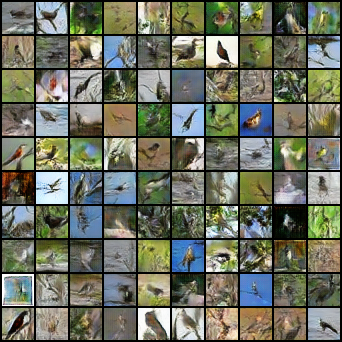
\includegraphics[width=.4\linewidth]{examples/samples_30000.png}
          \end{figure}
          \end{minipage}
    \end{itemize}
\item \textbf{Expected results:}
    \begin{itemize}
        \item Vanilla GAN: Final FID should be less than 110.
        \item LS-GAN: Final FID should be less than 90.
        \item WGAN-GP: Final FID should be less than 70.
    \end{itemize}
\item \textbf{Deliverables:} The code will log plots to \texttt{gan/data\_gan}, \texttt{gan/data\_ls\_gan}, and \texttt{gan/data\_wgan\_gp}. Extract plots and paste them into the appropriate section below. Note for all questions, we ask for final FID. Final FID is computed using 50K samples, at the very end of training. See the final printout for "Final FID  (Full 50K)". 
\end{itemize}
\newpage
\begin{questions}
\question Paste your plot of the samples and latent space interpolations from Vanilla GAN as well as the \textit{final} FID score you obtained. 
\begin{solution}
\\
Vanilla GAN FID: 
\\
\begin{figure}[H]
    \centering
    % TODO: put your plot here.
    \begin{subfigure}[b]{0.48\linewidth}
        \includegraphics[width=\linewidth]{example-image}
        \caption{Vanilla GAN Samples}
    \end{subfigure}
    \begin{subfigure}[b]{0.48\linewidth}
        \includegraphics[width=\linewidth]{example-image}
        \caption{Vanilla GAN Latent Space Interpolations}
    \end{subfigure}
\end{figure}
\end{solution}
\question Paste your plot of the samples and latent space interpolations from LS-GAN as well as the \textit{final} FID score you obtained. 
\begin{solution}
\\
LS-GAN FID: 
\\
\begin{figure}[H]
    \centering
    \begin{subfigure}[b]{0.48\linewidth}
        \includegraphics[width=\linewidth]{example-image}
        \caption{LS-GAN Samples}
    \end{subfigure}
    \begin{subfigure}[b]{0.48\linewidth}
        \includegraphics[width=\linewidth]{example-image}
        \caption{LS-GAN Latent Space Interpolations}
    \end{subfigure}
\end{figure}
\end{solution}
\question Paste your plot of the samples and latent space interpolations from WGAN-GP as well as the \textit{final} FID score you obtained. 
\\
\begin{solution}
\\
WGAN-GP FID:
\\
\begin{figure}[H]
    \centering
    \begin{subfigure}[b]{0.48\linewidth}
        \includegraphics[width=\linewidth]{example-image}
        \caption{WGAN-GP Samples}
    \end{subfigure}
    \begin{subfigure}[b]{0.48\linewidth}
        \includegraphics[width=\linewidth]{example-image}
        \caption{WGAN-GP Latent Space Interpolations}
    \end{subfigure}
\end{figure}  
\end{solution}
\end{questions}
\clearpage

\section{Variational Autoencoders (30 pts)}

We will be training Autoencoders and Variational Auto-Encoders (\href{https://arxiv.org/abs/1312.6114}{VAE}) on the \href{https://www.cs.toronto.edu/~kriz/cifar.html}{CIFAR-10} dataset.

\begin{itemize}
\item \textbf{Question:} Follow the instructions in the \texttt{README.md} file in the \texttt{vae/} folder to complete the implementation of VAEs.
\item \textbf{Debugging Tips:}
    \begin{itemize}
        \item Make sure the auto-encoder can produce good-quality reconstructions before moving on to the VAE. 
        While the VAE reconstructions might not be clear and the VAE samples even less so, the auto-encoder reconstructions should be very clear.
        \item If you are struggling to get the VAE portion working: debug the KL loss independently of the reconstruction loss to ensure the learned distribution matches standard normal. 
    \end{itemize}
\item \textbf{Expected results:}
    \begin{itemize}
        \item AE: reconstruction loss should be $<40$, reconstructions should look similar to original image.
        \item VAE: reconstruction loss should be $< 145$ ($\beta=1$ case).
        \item VAE: reconstruction loss should be $< 125$ when annealing $\beta$.
    \end{itemize}
\item \textbf{Deliverables:} The code will log plots to different folders in \texttt{vae}. Please paste the plots into the appropriate place for the questions below. Note for ALL questions, use the reconstructions and samples from the final epoch (epoch 19). 
\end{itemize}
\newpage
\begin{questions}
\question Autoencoder: For each latent size, paste your plot of the reconstruction loss curve and reconstructions.
\begin{solution}
\begin{figure}[H]
    \centering
    \begin{subfigure}[b]{0.32\linewidth}
    \includegraphics[width=\linewidth]{example-image}
    \caption{Loss (size 16)}
    \end{subfigure}
    \begin{subfigure}[b]{0.32\linewidth}
        \includegraphics[width=\linewidth]{example-image}
        \caption{Loss: (size 128)}
    \end{subfigure}
    \begin{subfigure}[b]{0.32\linewidth}
        \includegraphics[width=\linewidth]{example-image}
        \caption{Loss: (size 1024)}
    \end{subfigure}
    \begin{subfigure}[b]{0.32\linewidth}
    \includegraphics[width=\linewidth]{example-image}
    \caption{Reconstructions: (size 16)}
    \end{subfigure}
    \begin{subfigure}[b]{0.32\linewidth}
        \includegraphics[width=\linewidth]{example-image}
        \caption{Reconstructions: (size 128)}
    \end{subfigure}
    \begin{subfigure}[b]{0.32\linewidth}
        \includegraphics[width=\linewidth]{example-image}
        \caption{Reconstructions: (size 1024)}
    \end{subfigure}
\end{figure}
\end{solution}
\clearpage
\question VAE: Choose the $\beta$ that results in the best sample quality, $\beta^*$. Report the $\beta^*$ you used in your experiments. In addition, paste the reconstruction, KL loss curve plots, and the sample images corresponding to the VAE trained using constant $\beta^*$ and the VAE trained using $\beta$ annealing scheme with $\beta^*$.
\begin{solution}
\\
$\beta^*$ value:
\begin{figure}[H]
    \centering
    \begin{subfigure}[b]{0.32\linewidth}
    \includegraphics[width=\linewidth]{example-image}
    \caption{Recon. Loss: constant $\beta^*$}
    \end{subfigure}
    \begin{subfigure}[b]{0.32\linewidth}
    \includegraphics[width=\linewidth]{example-image}
    \caption{KL Loss: constant $\beta^*$}
    \end{subfigure}
    \begin{subfigure}[b]{0.32\linewidth}
    \includegraphics[width=\linewidth]{example-image}
    \caption{Samples: constant $\beta^*$}
    \end{subfigure}
    
    \begin{subfigure}[b]{0.32\linewidth}
    \includegraphics[width=\linewidth]{example-image}
    \caption{Recon. Loss: $\beta$ annealed}
    \end{subfigure}
    \begin{subfigure}[b]{0.32\linewidth}
    \includegraphics[width=\linewidth]{example-image}
    \caption{KL Loss: $\beta$ annealed}
    \end{subfigure}
    \begin{subfigure}[b]{0.32\linewidth}
    \includegraphics[width=\linewidth]{example-image}
    \caption{Samples: $\beta$ annealed}
    \end{subfigure}
\end{figure}
\end{solution}
\end{questions}
\newpage

\section{Diffusion Models (20 points)}
\begin{notebox}
\textbf{NOTE:} You only need to complete \textbf{ONE} of the following two sections: either Section 3 (Diffusion Models) OR Section 4 (Flow Matching Models). Both sections are worth 20 points.
\end{notebox}

We will be running inference using a pre-trained diffusion model (\href{https://arxiv.org/abs/2006.11239}{DDPM}) on CIFAR-10. 
\begin{itemize}
\item \textbf{Setup:} Download our pre-trained checkpoint for DDPM from \href{https://drive.google.com/file/d/1gtn9Jv9jBUol7iJw-94hw4j6KfpG3SZE/view?usp=sharing}{here}.
\item \textbf{Question:} Follow the instructions in the \texttt{README.md} file in the \texttt{diffusion/} folder to complete the implementation of the sampling procedures for Diffusion Models.
\item \textbf{Expected results:} 
    \begin{itemize}
        \item FID of less than 60 for DDPM and DDIM
    \end{itemize}
\item \textbf{Deliverables:} The code will log plots to \texttt{diffusion/data\_ddpm} and \texttt{diffusion/data\_ddim}. Extract plots and paste them into the appropriate section below. 
\end{itemize}
\begin{questions}
\question Paste your plots of the DDPM and DDIM samples.
\begin{solution}
\begin{figure}[H]
    \centering
    \begin{subfigure}[b]{0.48\linewidth}
        \includegraphics[width=\linewidth]{example-image}
        \caption{DDPM Samples}
    \end{subfigure}
    \begin{subfigure}[b]{0.48\linewidth}
        \includegraphics[width=\linewidth]{example-image}
        \caption{DDIM Samples}
    \end{subfigure}
\end{figure}
\end{solution}
\question Paste in the FID score you obtained from running inference using DDPM and DDIM.
\begin{solution}
\begin{itemize}
    \item DDPM FID:
    \item DDIM FID:
\end{itemize} 
\end{solution}
\question Compare the generated samples from your VAE and diffusion models. What do you observe? Does one generate better pictures than the other? Does the quality of the generated images match with the FID differences?
\begin{solution}
    \\
\end{solution}

\end{questions}

\newpage
\section{Flow Matching Models (20 points)}
\begin{notebox}
\textbf{NOTE:} You only need to complete \textbf{ONE} of the following two sections: either Section 3 (Diffusion Models) OR Section 4 (Flow Matching Models). Both sections are worth 20 points.
\end{notebox}

We will be running inference using a pre-trained flow matching model (\href{https://arxiv.org/abs/2210.02747}{flow matching}) on CIFAR-10. 
\begin{itemize}
\item \textbf{Setup:} Download our pre-trained checkpoint for flow matching model from \href{https://drive.google.com/file/d/16B8a_bElSnCLsNppTQOed7eUwsMcaxv6/view?usp=sharing}{here}.
\item \textbf{Question:} Follow the instructions in the \texttt{README.md} file in the \texttt{flow\_matching/} folder to complete the implementation of the sampling procedures for Flow Matching Models.
\item \textbf{Expected results:} 
    \begin{itemize}
        \item FID of less than 60 for Euler ODE sampling
    \end{itemize}
\item \textbf{Deliverables:} The code will log plots to \texttt{flow\_matching/flow\_euler}. Extract the plot and paste it into the section below. 
\end{itemize}
\begin{questions}
\question Paste your plots of the Euler ODE samples.
\begin{solution}
\begin{figure}[H]
    \centering
    \includegraphics[width=0.6\linewidth]{example-image}
    \caption{Flow Matching Euler ODE Samples}
\end{figure}
\end{solution}
\question Paste in the FID score you obtained from running inference using Euler ODE sampling.
\begin{solution}
\begin{itemize}
    \item Flow Matching FID:
\end{itemize} 
\end{solution}
\question Compare the generated samples from your VAE and flow matching models. What do you observe? Does one generate better pictures than the other?
\begin{solution}
    \\
\end{solution}

\end{questions}

\clearpage

\clearpage

\textbf{Collaboration Survey} Please answer the following:

\begin{enumerate}
    \item Did you receive any help whatsoever from anyone in solving this assignment?
    \begin{checkboxes}
     \choice Yes
     \choice No
    \end{checkboxes}
    \begin{itemize}
        \item If you answered `Yes', give full details:
        \item (e.g. “Jane Doe explained to me what is asked in Question 3.4”)
    \end{itemize}

    \begin{tcolorbox}[fit,height=3cm,blank, borderline={1pt}{-2pt},nobeforeafter]
    %Input your solution here.  Do not change any of the specifications of this solution box.
    \end{tcolorbox}

    \item Did you give any help whatsoever to anyone in solving this assignment?
    \begin{checkboxes}
     \choice Yes
     \choice No\
    \end{checkboxes}
    \begin{itemize}
        \item If you answered `Yes', give full details:
        \item (e.g. “I pointed Joe Smith to section 2.3 since he didn’t know how to proceed with Question 2”)
    \end{itemize}

    \begin{tcolorbox}[fit,height=3cm,blank, borderline={1pt}{-2pt},nobeforeafter]
    %Input your solution here.  Do not change any of the specifications of this solution box.
    \end{tcolorbox}

    \item Note that copying code or writeup even from a collaborator or anywhere on the internet violates the \href{hhttps://www.cmu.edu/policies/student-and-student-life/academic-integrity.html}{Academic Integrity Code of Conduct}.
\end{enumerate}

\end{document}